\documentclass[10pt]{article}

\usepackage[margin=0.75in]{geometry}
\usepackage{amsmath,amsthm,amssymb}
\usepackage{xcolor}
\usepackage{cancel}
\usepackage{graphicx}
\usepackage{changepage}
\usepackage{circuitikz}
\usepackage{pgfplots}
\usepackage{physics}
\usepackage{hyperref}
\usepackage{siunitx}
\usepackage[breakable]{tcolorbox}
\usepackage[inline]{enumitem}

\theoremstyle{definition}
\newtheorem{problem}{Problem}
\newtheorem{soln}{Solution}

\pgfplotsset{compat=newest}
\usetikzlibrary{lindenmayersystems}
\usetikzlibrary{arrows}

\definecolor{incolor}{HTML}{303F9F}
\definecolor{outcolor}{HTML}{D84315}
\definecolor{cellborder}{HTML}{CFCFCF}
\definecolor{cellbackground}{HTML}{F7F7F7}
\newcommand{\eq}{=}
\usetikzlibrary{positioning, fit, calc}
\pgfdeclarelayer{background}  
\pgfsetlayers{background,main}

\makeatletter
\newcommand{\boxspacing}{\kern\kvtcb@left@rule\kern\kvtcb@boxsep}
\makeatother
\newcommand{\prompt}[4]{
    \ttfamily\llap{{\color{#2}[#3]:\hspace{3pt}#4}}\vspace{-\baselineskip}
}

\newcommand{\thevenin}[2]{
  \begin{center}
    \begin{circuitikz} \draw
      (0,0) -- (2,0) to[battery1, l_=$V_{Th}\eq#1$] (2,2) 
      to[resistor, l_=$R_{Th}\eq#2$] (0,2)
      ;
      \draw [o-] (-.07,2.079);
      \draw [o-] (-.07,0.079);
    \end{circuitikz}
  \end{center}
}

\newcommand{\norton}[2]{
  \begin{center}
    \begin{circuitikz} \draw
      (0,0) -- (3,0) to[american current source, l_=$I_{N}\eq#1$] (3,2) -- (0,2) (2,0)
      to[resistor, l=$R_{N}\eq#2$] (2,2)
      ;
      \draw [o-] (-.07,2.079);
      \draw [o-] (-.07,0.079);
    \end{circuitikz}
  \end{center}
}

\newcommand{\highlight}[1]{\colorbox{yellow}{$\displaystyle #1$}}

\hypersetup{
    colorlinks=true,
    linkcolor=blue,
    filecolor=magenta,      
    urlcolor=cyan,
    pdftitle={Overleaf Example},
    pdfpagemode=FullScreen,
    }

\NewDocumentCommand{\evalat}{sO{\big}mm}{%
  \IfBooleanTF{#1}
   {\mleft. #3 \mright|_{#4}}
   {#3#2|_{#4}}%
}

\title{Physics 2250: Problem Set V}
\author{Jeremy Favro}
\date{\today}

\begin{document}

\maketitle

% PROBLEM 1
\begin{problem}
Consider the circuit below: $V_i$ is a periodic signal; $V_i=\left[1+8\cos(\omega t)\right]$.
\begin{center}
  \begin{circuitikz}[scale=0.85]
    \draw (0,0) to[american voltage source, l=$V_i\eq{\left[1+8\cos(\omega t)\right]}\unit{\volt}$, invert] ++(0,3)
    to[diode] ++(2.5,0) to[resistor, l=$R\eq1\unit{\kilo\ohm}$] ++(2.5,0) -- ++(1, 0) node[right]{$V_o$}
    ++(-1,0) to[ammeter] ++(0,-1.5) to[battery1, l=$V\eq3\unit{\volt}$] ++(0,-1.5) node[ground]{} -- (0,0)
    ;
  \end{circuitikz}
\end{center}
\end{problem}
\begin{soln} a \& b)
  \begin{center}
    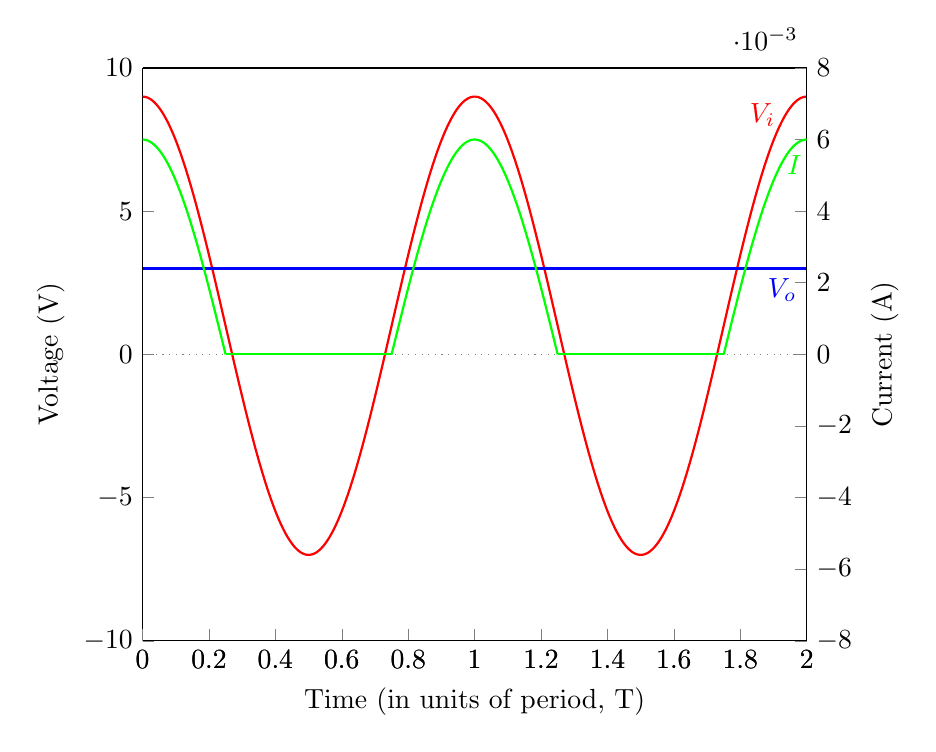
\begin{tikzpicture}[scale = 1]
      \pgfplotsset{
        scale only axis,
        xmin=0, xmax=2
      }
      \begin{axis}[
          axis y line*=left,
          ymin=-10, ymax=10,
          xlabel={Time (in units of period, T)},
          ylabel={Voltage ($\unit{\volt}$)},
          xtick pos=left,
          ytick pos=left
        ]
        
        \addplot[thick,red,samples=500,domain=0:2] (\x,{1+8*cos((2*pi*\x)*180/pi)}) node[pos=0.99, left]{$V_i$};
        \addplot[thick,blue,samples=2,domain=0:2] (\x,{3}) node[below left]{$V_o$};
        \addplot[gray,dotted,samples=2,domain=0:2] (\x,{0});
        
      \end{axis}
      
      \begin{axis}[
          axis y line*=right,
          ymin=-8*10^-3, ymax=8*10^-3,
          ylabel={Current ($\unit{\ampere}$)},
          xtick pos=left,
          ytick pos=right
        ]
        \addplot[thick,green,samples=500,domain=0:1/4] (\x,{6/1000*cos((2*pi*\x)*180/pi)});
        \addplot[thick,green,samples=500,domain=1/4:3/4] (\x,{0});
        \addplot[thick,green,samples=500,domain=3/4:5/4] (\x,{6/1000*cos((2*pi*\x)*180/pi)});
        \addplot[thick,green,samples=500,domain=5/4:7/4] (\x,{0});
        \addplot[thick,green,samples=500,domain=7/4:8/4] (\x,{6/1000*cos((2*pi*\x)*180/pi)}) node[pos=0.85, below]{$I$};
        
      \end{axis}
    \end{tikzpicture}
  \end{center}
  $V_o$ and $V_i$ are effectively given by the problem. $I$ (at peak) is given by $\displaystyle\frac{V_i-V}{R}=6\unit{\milli\ampere}$ because the two sources will ``fight''
  when the diode is maximally forward-biased. When the diode is reverse-biased, there will be no current whatsoever as both sources will cooperate and try to push current backwards
  across the diode.
\end{soln}
\newpage

% PROBLEM 2
\begin{problem}
Determine the current passing through each of the three diodes in the circuit shown below. 
\begin{center}
  \begin{circuitikz}[scale=0.85]
    \draw (0,4.5) to[battery1, l_=$V_S\eq20\unit{\volt}$] ++(0,-4.5) ++(0,4.5)
    to[diode, l=$D_1$] ++(1.5,0) to[battery1, l_=$V_d\eq0.7\unit{\volt}$] ++(1.5,0) to[resistor, l=$R_o\eq20\unit{\ohm}$] ++(1.5, 0) 
    to[diode, l=$D_2$] ++(0,-1.5) to[battery1, l_=$V_d\eq0.7\unit{\volt}$] ++(0,-1.5) to[resistor, l_=$R_o\eq20\unit{\ohm}$] ++(0,-1.5) 
    to[resistor, l_=$R_1\eq2\unit{\kilo\ohm}$] ++(3,0)
    to[diode, l=$D_3$] ++(0,1.5) to[battery1, l=$V_d\eq0.7\unit{\volt}$] ++(0,1.5) to[resistor, l=$R_o\eq20\unit{\ohm}$] ++(0,1.5)
    -- ++(-3,0) (0,0) to[resistor, l_=$R_2\eq1\unit{\kilo\ohm}$] ++(4.5,0)
    ;
  \end{circuitikz}
\end{center}
\end{problem}
\begin{soln} Right off the bat $D_3$ is reverse-biased so sees no current. This leaves a simple single-loop circuit (through which current is conserved) so
  \begin{align*}
     & 0=20\unit{\volt}-0.7\unit{\volt}-IR_o-0.7\unit{\volt}-IR_o-IR_2             \\
     & \frac{1.4\unit{\volt}-20\unit{\volt}}{-2R_o-R_2}=I\approxeq9.12\unit{\milli\ampere}
  \end{align*}
  So $D_1$ and $D_2$ experience a current of $\approx9.12\unit{\milli\ampere}$ and $D_3$ experiences no current (because it is reverse-biased).
\end{soln}

% PROBLEM 3
\begin{problem}
Determine the current passing through each of the three diodes in the circuit shown below. 
\begin{center}
  \begin{circuitikz}[scale=0.85]
    \draw (0,4.5) to[battery1, l_=$V_S\eq25\unit{\volt}$] ++(0,-4.5) ++(0,4.5)
    to[resistor, l=$R_1\eq50\unit{\ohm}$] ++(2,0) coordinate(J1) to[resistor, l=$R_4\eq60\unit{\ohm}$, -*] ++(3,0)
    to[diode] ++(0,-1.5) to[battery1, l=$V_d\eq0.7\unit{\volt}$] ++(0,-1.5) to[resistor, l=$R_o\eq20\unit{\ohm}$] ++(0,-1.5)
    -- ++(-3,0) to[resistor, l=$R_3\eq150\unit{\ohm}$] (0,0) (J1) to[resistor, l=$R_2\eq50\unit{\ohm}$] ++(0,-4.5)
    ;
  \end{circuitikz}
\end{center}
\end{problem}
\begin{soln} Because the $V_d$ source can push no current through the diode the total current is given by $I=\displaystyle\frac{V_S}{R_1+R_3+\left(R_2^{-1}+\left[R_4+R_o\right]^{-1}\right)^{-1}}=\frac{13}{120}\unit{\ampere}$.
  This current is split between the $R_2$ and $R_4$ branches by the current divider $I_{R4}=\displaystyle I\frac{R_2}{R_4+R_2+R_o}=\frac{1}{24}\unit{\ampere}$ so the power dissipated by
  $R_o$ is $P=I_{R_4}^2R_o\approxeq34.7\unit{\milli\watt}$.
\end{soln}
\newpage

% PROBLEM 4
\begin{problem}
Consider a sinusoidal voltage supply with $V_S=\displaystyle \left[20\sin\left(\frac{2\pi}{T}t\right)\right]\unit{\volt}$ and a resistance $R_S=1\unit{\kilo\ohm}$, as shown in the figure below.
\begin{center}
  \begin{circuitikz}[scale=0.85]
    \draw (0,2) to[battery1, l_=$V_S\eq\displaystyle {\left[20\sin\left(\frac{2\pi}{T}t\right)\right]}\unit{\volt}$] ++(0,-2) ++(0,2)
    to[resistor, l=$R_1\eq1\unit{\kilo\ohm}$] ++(2,0) (0,0) node[ground]{}
    ;
  \end{circuitikz}
\end{center}
\end{problem}
\begin{soln} ~\\
  a) To transform the given $V_S$ into the desired $V_o$ we need to invert it, triple it, and clip the positive voltages. To do this we can make use of an op amp in the
  inverting configuration and a diode that is reverse biased when the output of that op amp (three times the negative of the input voltage) is greater than zero.
  \begin{center}
    \begin{circuitikz}
      \draw (0,2) to[battery1, l_=$V_S\eq\displaystyle {\left[20\sin\left(\frac{2\pi}{T}t\right)\right]}\unit{\volt}$] ++(0,-2) ++(0,2)
      to[resistor, l=$R_S\eq1\unit{\kilo\ohm}$] ++(2,0) coordinate(S) (0,0) coordinate (G) node[ground]{}
      (S) node[op amp, scale=0.75, anchor=-](A){A}
      (A.-) -- ++(0,1) coordinate(RF) to[resistor, l=$R_f\eq3\unit{\kilo\ohm}$] (RF -| A.out) -- (A.out)
      to[diode, invert] ++(1,0) node[right]{$V_o$}
      (A.+) -- (G -| A.+) -- (G)
      ;
    \end{circuitikz}
  \end{center}
    b) We can reuse the logic behind the first circuit but we now need to offset the voltage drop across the now non-ideal diode and figure out a way to recreate the $3:1$ resistor ratio.
    We can offset the diode voltage drop with a $0.2\unit{\volt}$ battery and a $0.5\unit{\volt}$ battery in series and we can recreate the $3\unit{\kilo\ohm}$ resistor
    by using a pair of $1\unit{\kilo\ohm}$ and $5\unit{\kilo\ohm}$ resistors in parallel.
    \begin{center}
      \begin{circuitikz}
        \draw (0,2) to[battery1, l_=$V_S\eq\displaystyle {\left[20\sin\left(\frac{2\pi}{T}t\right)\right]}\unit{\volt}$] ++(0,-2) ++(0,2)
        to[resistor, l=$R_S\eq1\unit{\kilo\ohm}$] ++(2,0) coordinate(S) (0,0) coordinate (G) node[ground]{}
        (S) ++(1.5,0) node[op amp, scale=0.75, anchor=-](A){A}
        (S) -- (A.-) (S) -- ++(0,1) coordinate(RF) to[resistor, l=$1\unit{\kilo\ohm}$] ++(1.5, 0) to[resistor, l=$5\unit{\kilo\ohm}$] (RF -| A.out) coordinate(RJO) -- (A.out)
        (S) ++(0,1) -- ++(0,1) coordinate(RF2) to[resistor, l=$1\unit{\kilo\ohm}$] ++(1.5, 0) to[resistor, l=$5\unit{\kilo\ohm}$] (RF2 -| A.out) -- (RJO) (A.out)
        to[battery1, l_=$0.2\unit{\volt}$] ++(0.5,0) to[battery1, l=$0.5\unit{\volt}$] ++(0.5,0) coordinate(D) ++(1,0) to[diode, l=Si] (D) ++(1,0) node[right]{$V_o$}
        (A.+) -- (G -| A.+) -- (G)
        ;
      \end{circuitikz}
    \end{center}
  Both a) and b) assume that the op amps have no maximum (or minimum) voltage output because I can't think of a way to create the required amplification otherwise.
\end{soln}
\end{document}